\chapter{Reactiesnelheden}\label{ch:g12:reaction-rates}

Een fles melk die op het aanrecht blijft staan, is in een paar dagen
zuur; in de koelkast blijft ze meer dan een week goed. Vuurwerk verbrandt
in een fractie van een seconde, terwijl een kalkstenen beeld in een
stadspark in eeuwen verweert. \omterm{def:g8:balanced-equations:equation}{Kloppende reactievergelijkingen} en
\omterm{def:g10:reaction-progress-table:extent}{voortgangstabellen} zeggen wat een reactie oplevert en hoeveel; ze zeggen
niets over hoe snel. Dit hoofdstuk meet de snelheid van reacties, zoekt
uit wat die bepaalt, en beschrijft de eenvoudigste manier waarop een
reactie onderweg vertraagt.

\begin{recall}
De concentratie van een oplossing (\cref{ch:g10:concentration-and-dilution})
en de voortgang van een reactie (\cref{ch:g10:reaction-progress-table}). De
\omterm{def:g11:absorbance:absorbance}{absorbantie} van een verdunde oplossing is evenredig met de concentratie
van het gekleurde deeltje (\cref{ch:g11:absorbance}). Een \omterm{def:g11:titration:titration}{titratie} meet de
hoeveelheid van een deeltje (\cref{ch:g11:titration}).
\end{recall}

\begin{omfigure}
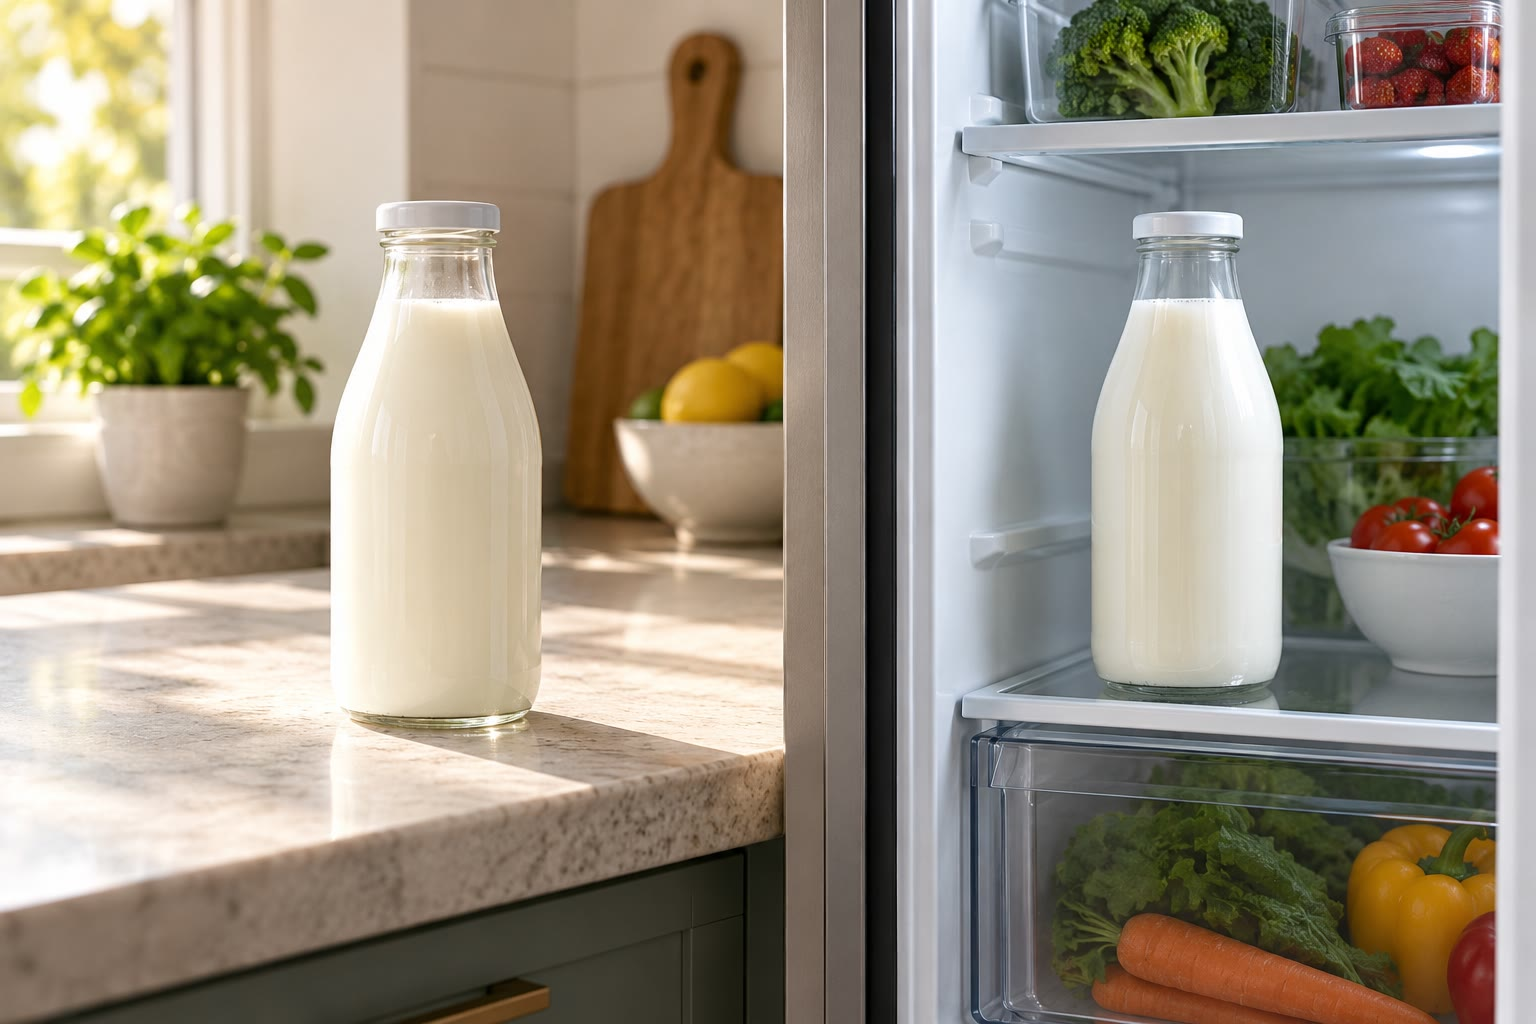
\includegraphics[width=0.48\linewidth]{images/book1/ai/g12-milk-counter-fridge.jpg}

{\small Dezelfde melk, op het aanrecht en in de koelkast: de reacties
waardoor ze zuur wordt, verlopen in de kou langzamer.}
\end{omfigure}

\section{Een reactie in de tijd volgen}

Sommige reacties zijn voorbij zodra de \omterm{def:g7:chemical-reactions:reactant}{beginstoffen} elkaar ontmoeten: het
neerslaan van zilverchloride, de reactie van een zuur met een base.
Andere duren minuten, uren of jaren. Om een langzame reactie te
bestuderen, meten scheikundigen op vaste tijdstippen de concentratie van
een \omterm{def:g7:chemical-reactions:reactant}{beginstof} of een \omterm{def:g7:chemical-reactions:reactant}{reactieproduct}. Ze kunnen
\begin{itemize}
  \item kleine monsters nemen, in elk monster de reactie stoppen, en ze
        titreren;
  \item de \omterm{def:g11:absorbance:absorbance}{absorbantie} van de oplossing meten, als een \omterm{def:g7:chemical-reactions:reactant}{beginstof} of een
        \omterm{def:g7:chemical-reactions:reactant}{reactieproduct} gekleurd is;
  \item de druk of het volume van een gas dat vrijkomt meten, of de
        geleidbaarheid van een oplossing waarvan de \omterm{def:g9:ions:ion}{ionen} veranderen.
\end{itemize}

\begin{definition}[Afschrikken]\label{def:g12:reaction-rates:quenching}
Een monster \emph{afschrikken}\index{afschrikken} is de reactie erin
stoppen, of heel sterk vertragen, op het moment dat het genomen wordt,
meestal door het plotseling af te koelen en te verdunnen, zodat je de
samenstelling op je gemak kunt meten.
\end{definition}

\begin{inthelab}[Een monster afschrikken]
Om de vijf minuten wordt met een pipet \qty{10.0}{mL} van het
reactiemengsel genomen en in een bekerglas met ongeveer \qty{40}{mL}
ijskoud water gegoten. Vijf keer verdund en afgekoeld tot dicht bij
\qty{0}{\celsius} wordt de reactie zo langzaam dat je haar als gestopt
kunt beschouwen; daarna wordt het monster getitreerd. Het tijdstip van het
monster is het moment waarop het in het ijswater werd gegoten, niet het
moment van de \omterm{def:g11:titration:titration}{titratie}.
\end{inthelab}

\begin{omfigure}
\begin{tikzpicture}[font=\small, scale=0.8]
  \pic[transform shape] at (0,0) {erlenmeyer={0.4}{orange!25}};
  \node[anchor=north, align=center] at (0,-0.15) {reactie-\\ mengsel};
  \pic[transform shape, rotate=-35] at (1.4,1.2) {pipette={0.6}{orange!25}};
  \draw[omProp, very thick, -{Stealth}] (1.6,0.8) -- (2.9,0.8);
  \node[anchor=south] at (2.25,0.85) {\qty{10.0}{mL}};
  \pic[transform shape] at (4,0) {beaker={0.55}{cyan!12}};
  \foreach \p in {(3.6,0.4),(4.2,0.6),(3.9,0.85),(4.4,0.3)}
    \draw[black!30, fill=white] \p ++(-0.1,-0.08) rectangle ++(0.2,0.16);
  \node[anchor=north, align=center] at (4,-0.15) {ijskoud water:\\ reactie gestopt};
  \draw[omProp, very thick, -{Stealth}] (5.1,0.8) -- (6.4,0.8);
  \pic[transform shape] at (7.5,0) {erlenmeyer={0.35}{orange!12}};
  \pic[transform shape] at (7.5,2.75) {burette={0.7}{violet!45}};
  \node[anchor=north, align=center] at (7.5,-0.15) {titratie van\\ het monster};
\end{tikzpicture}

{\small Een reactie volgen met monsters: neem een monster, schrik het af,
en meet het daarna op je gemak.}
\end{omfigure}

\section{Kinetische factoren}

\begin{definition}[Kinetische factor]\label{def:g12:reaction-rates:kinetic-factor}
Een \emph{kinetische factor}\index{kinetische factor} is een grootheid die
de snelheid van een reactie verandert zonder te veranderen wat de reactie
oplevert: de temperatuur, de concentraties van de \omterm{def:g7:chemical-reactions:reactant}{beginstoffen}, het
contactoppervlak tussen \omterm{def:g7:chemical-reactions:reactant}{beginstoffen} in verschillende fasen, en de
aanwezigheid van een katalysator (volgend hoofdstuk).
\end{definition}

\begin{proposition}[Warmer, geconcentreerder, fijner: sneller]\label{prop:g12:reaction-rates:factors}
In het algemeen is een reactie sneller als de temperatuur hoger is, als
de \omterm{def:g7:chemical-reactions:reactant}{beginstoffen} geconcentreerder zijn, en, bij een vaste \omterm{def:g7:chemical-reactions:reactant}{beginstof}, als
die fijner verdeeld is.
\end{proposition}

\begin{proof}
Aangenomen, met een beeld: deeltjes die reageren, moeten elkaar
ontmoeten, en hard genoeg. Ze concentreren maakt ontmoetingen frequenter;
een vaste stof verdelen biedt meer oppervlak om elkaar te ontmoeten;
verwarmen laat ze sneller bewegen, zodat ze elkaar vaker ontmoeten en,
vooral, meer van de ontmoetingen energiek genoeg zijn om bindingen te
verbreken.
\end{proof}

\begin{example}[Drie gevallen uit het dagelijks leven]\label{ex:g12:reaction-rates:everyday}
Voedsel blijft langer goed in de koelkast en veel langer in de vriezer:
de reacties die het bederven, vertragen in de kou. Fijn meelstof in de
\omterm{def:g4:air-a-mixture-of-gases:air}{lucht} van een \omterm{def:g10:the-mole:amount}{molen} kan ontploffen, terwijl een zak meel alleen
smeult: dezelfde reactie, een enorm contactoppervlak. Een bruistablet lost
sneller op in water als je hem eerst fijnmaakt.
\end{example}

\begin{omfigure}
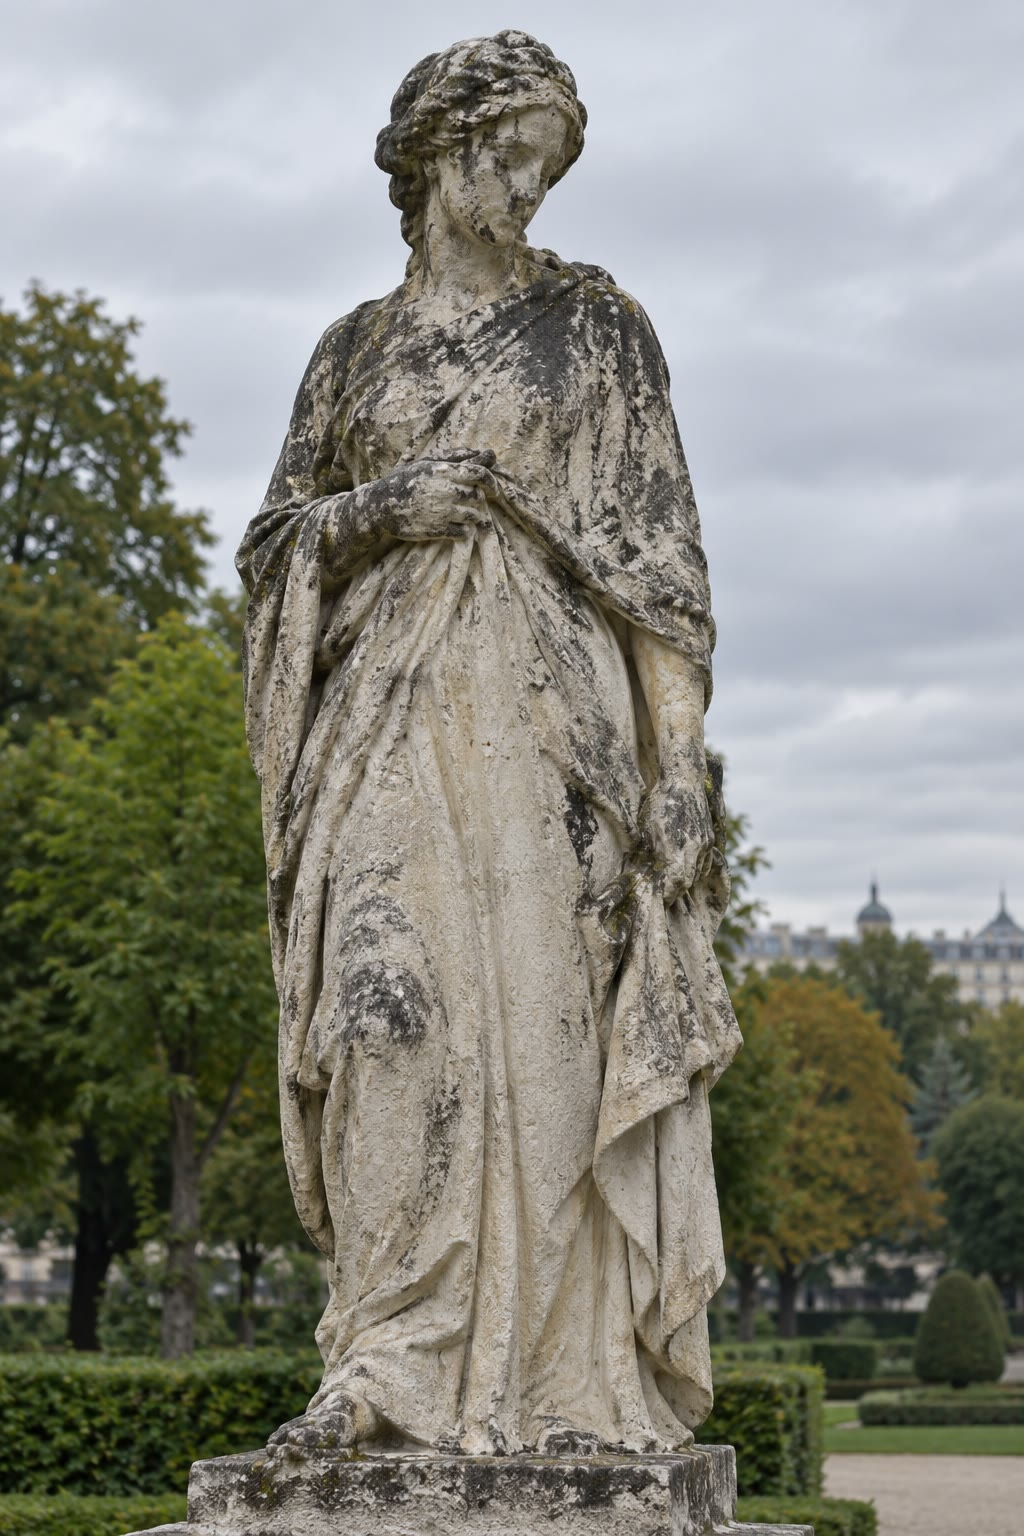
\includegraphics[width=0.42\linewidth,height=6cm,keepaspectratio]{images/book1/ai/g12-weathered-statue.jpg}

{\small Een kalkstenen beeld dat door de regen verweerd is: een reactie
die eeuwen duurt.}
\end{omfigure}

\section{Verdwijningssnelheid en vormingssnelheid}

\begin{definition}[Verdwijningssnelheid, vormingssnelheid]\label{def:g12:reaction-rates:rate}
In een oplossing met een constant volume is de
\emph{verdwijningssnelheid}\index{verdwijningssnelheid}
van een \omterm{def:g7:chemical-reactions:reactant}{beginstof} A op tijdstip $t$
\[
  v_A(t) = -\frac{d[\ce{A}]}{dt},
\]
en de \emph{vormingssnelheid}\index{vormingssnelheid} van een
\omterm{def:g7:chemical-reactions:reactant}{reactieproduct} P is $v_P(t) = \dfrac{d[\ce{P}]}{dt}$. Beide zijn positief,
in \si{mol.L^{-1}.min^{-1}} (of per seconde).
\end{definition}


\begin{method}[Een snelheid aflezen met een raaklijn]\label{met:g12:reaction-rates:tangent}
\begin{enumerate}
  \item Teken in de grafiek van $[\ce{A}]$ tegen $t$ de raaklijn op het
        gekozen tijdstip.
  \item Lees twee punten ver uit elkaar op de raaklijn af en bereken haar
        helling, $\Delta[\ce{A}] / \Delta t$.
  \item De \omterm{def:g12:reaction-rates:rate}{verdwijningssnelheid} is het tegengestelde van deze helling
        (voor een \omterm{def:g7:chemical-reactions:reactant}{reactieproduct} de helling zelf).
\end{enumerate}
\end{method}

\begin{omfigure}
\begin{tikzpicture}
\begin{axis}[width=0.8\linewidth, height=6.4cm, xmin=0, xmax=60, ymin=0,
    ymax=11, xlabel={$t$ (\si{min})}, ylabel={$[\ce{A}]$ (\si{mmol/L})},
    axis lines*=left, ymajorgrids, xmajorgrids, grid style={gray!20},
    tick label style={font=\small}, label style={font=\small},
    legend style={font=\small, at={(0.98,0.97)}, anchor=north east,
    draw=none, fill=white}, legend cell align=left]
  \addplot[very thick, omDef] table[x=t, y=A1] {figdata/out/grade-12-reaction-rates-a.dat};
  \addplot[very thick, omThm] table[x=t, y=A2] {figdata/out/grade-12-reaction-rates-a.dat};
  \addplot[thick, dashed, omProp, restrict y to domain=0:11] table[x=t, y=tangent]
    {figdata/out/grade-12-reaction-rates-a.dat};
  \legend{$k = \qty{0.050}{min^{-1}}$, $k = \qty{0.100}{min^{-1}}$ (warmer),
    raaklijn bij $t = 0$}
  \addplot[densely dotted, black!60] coordinates {(0,5) (13.86,5) (13.86,0)};
  \addplot[densely dotted, black!60] coordinates {(6.93,5) (6.93,0)};
  \node[font=\small, anchor=south west] at (axis cs:14.6,5.4) {$t_{1/2} = \qty{13.9}{min}$};
  \node[font=\small, anchor=south east] at (axis cs:6.7,0.2) {\qty{6.9}{min}};
\end{axis}
\end{tikzpicture}

{\small De concentratie van een \omterm{def:g7:chemical-reactions:reactant}{beginstof} A tegen de tijd, voor dezelfde
\omterm{def:g12:reaction-rates:first-order}{eerste-ordereactie} bij twee temperaturen. De raaklijn bij $t = 0$
(gestreept) geeft de beginsnelheid; de gestippelde lijnen geven de
\omterm{def:g12:reaction-rates:half-life}{halveringstijden} aan.}
\end{omfigure}

\begin{example}[De beginsnelheid]\label{ex:g12:reaction-rates:initial}
Op de blauwe kromme gaat de raaklijn bij $t = 0$ van \qty{10.0}{mmol/L}
bij $t = 0$ naar $0$ bij $t = \qty{20}{min}$: haar helling is
$-10.0/20 = \qty{-0.50}{mmol.L^{-1}.min^{-1}}$, dus de beginsnelheid van
verdwijnen is \qty{0.50}{mmol.L^{-1}.min^{-1}}. Later vlakt de kromme af
en daalt de snelheid: de reactie vertraagt naarmate A opraakt.
\end{example}

\section{Eerste-ordereacties}

\begin{definition}[Eerste-ordereactie, snelheidsconstante]\label{def:g12:reaction-rates:first-order}
Een reactie is een \emph{eerste-ordereactie}\index{eerste-ordereactie}
in A als haar \omterm{def:g12:reaction-rates:rate}{verdwijningssnelheid} op elk moment evenredig is met de
concentratie van A:
\[
  -\frac{d[\ce{A}]}{dt} = k\,[\ce{A}] .
\]
De positieve constante $k$, in \si{min^{-1}} of \si{s^{-1}}, is de
\emph{snelheidsconstante}\index{snelheidsconstante}; ze hangt af van de
temperatuur.
\end{definition}

\begin{proposition}[Exponentiële afname]\label{prop:g12:reaction-rates:exponential}
Voor een \omterm{def:g12:reaction-rates:first-order}{eerste-ordereactie} met beginconcentratie $[\ce{A}]_0$ geldt
\[
  [\ce{A}](t) = [\ce{A}]_0\, e^{-kt} .
\]
\end{proposition}

\begin{proof}
De functie $f(t) = [\ce{A}]_0 e^{-kt}$ heeft als afgeleide
$f'(t) = -k [\ce{A}]_0 e^{-kt} = -k f(t)$, dus ze voldoet aan de
snelheidsvergelijking, en $f(0) = [\ce{A}]_0$. Dat het de enige zulke
functie is, wordt hier aangenomen (het wordt in de wiskunde bewezen, voor
vergelijkingen $y' = ay$).
\end{proof}

\begin{method}[Testen op eerste orde]\label{met:g12:reaction-rates:test}
\begin{enumerate}
  \item Bereken uit de metingen op elk tijdstip $\ln [\ce{A}]$ (of
        $\ln A$ voor een \omterm{def:g11:absorbance:absorbance}{absorbantie} die evenredig is met $[\ce{A}]$).
  \item Zet $\ln[\ce{A}]$ uit tegen $t$: omdat
        $\ln[\ce{A}] = \ln[\ce{A}]_0 - kt$, liggen de punten op een rechte
        lijn dan en slechts dan als de reactie van de eerste orde is.
  \item De helling van de lijn is $-k$.
\end{enumerate}
\end{method}

\section{Halveringstijd}

\begin{definition}[Halveringstijd]\label{def:g12:reaction-rates:half-life}
De \emph{halveringstijd}\index{halveringstijd} $t_{1/2}$ van een reactie
is de tijd die de concentratie van de \omterm{def:g10:reaction-progress-table:limiting}{beperkende beginstof} nodig heeft om
tot de helft van haar beginwaarde te dalen.
\end{definition}

\begin{proposition}[Halveringstijd van een eerste-ordereactie]\label{prop:g12:reaction-rates:half-life}
Voor een \omterm{def:g12:reaction-rates:first-order}{eerste-ordereactie} geldt
\[
  t_{1/2} = \frac{\ln 2}{k},
\]
wat de beginconcentratie ook is; na $n$ \omterm{def:g12:reaction-rates:half-life}{halveringstijden} is de
concentratie gedeeld door $2^n$.
\end{proposition}

\begin{proof}
$[\ce{A}]_0 e^{-k t_{1/2}} = [\ce{A}]_0 / 2$ geeft $e^{-k t_{1/2}} = 1/2$,
dus $k t_{1/2} = \ln 2$. Elke volgende \omterm{def:g12:reaction-rates:half-life}{halveringstijd} vermenigvuldigt de
concentratie opnieuw met $e^{-k t_{1/2}} = 1/2$.
\end{proof}


\begin{example}[De halveringstijden aflezen]\label{ex:g12:reaction-rates:half-lives}
Voor $k = \qty{0.050}{min^{-1}}$ is $t_{1/2} = 0.693 / 0.050 =
\qty{13.9}{min}$: de concentratie daalt van 10.0 naar 5.0, dan 2.5,
dan \qty{1.25}{mmol/L} bij 13.9, 27.7 en \qty{41.6}{min}. De warmere
proef, met een twee keer zo grote $k$, heeft de halve \omterm{def:g12:reaction-rates:half-life}{halveringstijd},
\qty{6.9}{min}, zoals de figuur laat zien.
\end{example}

\begin{remark}[Halveringstijden elders]\label{rem:g12:reaction-rates:radioactive}
Hetzelfde woord wordt in de natuurkunde gebruikt voor radioactieve kernen,
waarvan het aantal op dezelfde exponentiële manier afneemt: radioactief
verval gedraagt zich als een \omterm{def:g12:reaction-rates:first-order}{eerste-ordereactie}. Het natuurkundeboek
behandelt het.
\end{remark}

\begin{omfigure}
\begin{minipage}{0.49\linewidth}
\begin{tikzpicture}
\begin{axis}[width=\linewidth, height=5.4cm, xmin=0, xmax=26, ymin=0,
    ymax=0.85, xlabel={$t$ (\si{min})}, ylabel={absorbantie $A$},
    axis lines*=left, ymajorgrids, grid style={gray!20},
    tick label style={font=\scriptsize}, label style={font=\small}]
  \addplot[only marks, mark=*, mark size=1.8pt, omDef] table[x=t, y=A]
    {figdata/out/grade-12-reaction-rates-b.dat};
  \addplot[thick, omProp, domain=0:26, samples=60] {0.8*exp(-0.11552*x)};
\end{axis}
\end{tikzpicture}
\end{minipage}\hfill
\begin{minipage}{0.49\linewidth}
\begin{tikzpicture}
\begin{axis}[width=\linewidth, height=5.4cm, xmin=0, xmax=26, ymin=-3.4,
    ymax=0, xlabel={$t$ (\si{min})}, ylabel={$\ln A$}, axis lines*=left,
    ymajorgrids, grid style={gray!20}, tick label style={font=\scriptsize},
    label style={font=\small}]
  \addplot[only marks, mark=*, mark size=1.8pt, omDef] table[x=t, y=lnA]
    {figdata/out/grade-12-reaction-rates-b.dat};
  \addplot[thick, omProp, domain=0:26] {-0.2231-0.11552*x};
\end{axis}
\end{tikzpicture}
\end{minipage}


{\small Het verbleken van kristalviolet in een \omterm{def:g9:acids-bases-ph:acidic}{basische oplossing}
(gegevens van het weekendprobleem). Links: de \omterm{def:g11:absorbance:absorbance}{absorbantie} daalt langs een
exponentiële kromme. Rechts: $\ln A$ tegen $t$ is een rechte lijn met
helling $-\qty{0.116}{min^{-1}}$: de reactie is van de eerste orde in de
kleurstof.}
\end{omfigure}

\section{Oefeningen}

\begin{exercise}[$\star$]\label{exo:g12:reaction-rates:1}
Noem de \omterm{def:g12:reaction-rates:kinetic-factor}{kinetische factor} die in elk geval werkt: een koelkast houdt
voedsel goed; poedersuiker lost sneller op dan een suikerklontje; een
geconcentreerder zuur tast zink sneller aan; een doorgesneden appel wordt in de
zomer sneller bruin.
\end{exercise}

\begin{exercise}[$\star$]\label{exo:g12:reaction-rates:2}
Lees in de figuur van $[\ce{A}]$ tegen de tijd de \omterm{def:g12:reaction-rates:half-life}{halveringstijd} van elke
proef af. Wat is $[\ce{A}]$ op de blauwe kromme na twee \omterm{def:g12:reaction-rates:half-life}{halveringstijden}?
\end{exercise}

\begin{exercise}[$\star$]\label{exo:g12:reaction-rates:3}
Een raaklijn aan de kromme van een \omterm{def:g7:chemical-reactions:reactant}{reactieproduct}, getekend bij
$t = \qty{5}{min}$, gaat door $(0, \qty{1.0}{mmol/L})$ en
$(\qty{10}{min}, \qty{5.0}{mmol/L})$. Wat is de \omterm{def:g12:reaction-rates:rate}{vormingssnelheid} van het
product bij \qty{5}{min}?
\end{exercise}

\begin{exercise}[$\star$]\label{exo:g12:reaction-rates:4}
Waarom wordt een monster in ijskoud water gegoten voordat het getitreerd
wordt? Waarom moet het tijdstip van het monster genoteerd worden als het
wordt uitgegoten, en niet als het wordt getitreerd?
\end{exercise}

\begin{exercise}[$\star$]\label{exo:g12:reaction-rates:5}
Een \omterm{def:g12:reaction-rates:first-order}{eerste-ordereactie} heeft een \omterm{def:g12:reaction-rates:half-life}{halveringstijd} van \qty{10}{min}. Welk
deel van de \omterm{def:g7:chemical-reactions:reactant}{beginstof} is er na \qty{30}{min} nog over? En na \qty{1}{h}?
\end{exercise}

\begin{exercise}[$\star\star$]\label{exo:g12:reaction-rates:6}
Concentraties van een \omterm{def:g7:chemical-reactions:reactant}{beginstof}, in \si{mmol/L}: 8.00 bij \qty{0}{min},
5.66 bij \qty{5}{min}, 4.00 bij \qty{10}{min}, 2.83 bij \qty{15}{min},
2.00 bij \qty{20}{min}. Bereken op elk tijdstip $\ln[\ce{A}]$ en laat zien
dat de reactie van de eerste orde is. Bepaal $k$ en de \omterm{def:g12:reaction-rates:half-life}{halveringstijd}.
\end{exercise}

\begin{exercise}[$\star\star$]\label{exo:g12:reaction-rates:7}
Een \omterm{def:g12:reaction-rates:first-order}{eerste-ordereactie} heeft $t_{1/2} = \qty{25}{s}$. Bereken $k$.
\end{exercise}

\begin{exercise}[$\star\star$]\label{exo:g12:reaction-rates:8}
Bereken voor $[\ce{A}]_0 = \qty{0.100}{mol/L}$ en
$k = \qty{0.020}{min^{-1}}$ de concentratie $[\ce{A}]$ na 10, 30 en
\qty{100}{min}.
\end{exercise}

\begin{exercise}[$\star\star$]\label{exo:g12:reaction-rates:9}
Schat in de figuur van $[\ce{A}]$ tegen de tijd de helling van de blauwe
kromme bij $t = \qty{13.9}{min}$ (teken een raaklijn), en vergelijk die
met $-k[\ce{A}]$ op dat tijdstip.
\end{exercise}

\begin{exercise}[$\star\star$]\label{exo:g12:reaction-rates:10}
Jood \ce{I2}, bruin, ontstaat langzaam in een kleurloze oplossing. De
\omterm{def:g11:absorbance:absorbance}{absorbantie} stijgt van 0 naar 0.60. Leg uit waarom je de \omterm{def:g11:absorbance:absorbance}{absorbantie} kunt
gebruiken om $[\ce{I2}]$ te volgen, en hoe je de \omterm{def:g12:reaction-rates:rate}{vormingssnelheid} op een
gegeven tijdstip afleest in de grafiek van $A$ tegen $t$.
\end{exercise}

\begin{exercise}[$\star\star$]\label{exo:g12:reaction-rates:11}
Twee proeven met dezelfde reactie beginnen bij $[\ce{A}]_0 = 10$ en
\qty{20}{mmol/L}. Vergelijk, als de reactie van de eerste orde is, hun
beginsnelheden en hun \omterm{def:g12:reaction-rates:half-life}{halveringstijden}.
\end{exercise}

\begin{exercise}[$\star\star\star$]\label{exo:g12:reaction-rates:12}
Hoeveel \omterm{def:g12:reaction-rates:half-life}{halveringstijden} heeft een \omterm{def:g12:reaction-rates:first-order}{eerste-ordereactie} nodig om op
\qty{1}{\percent} van haar \omterm{def:g7:chemical-reactions:reactant}{beginstof} uit te komen? En op
\qty{0.1}{\percent}? Geef de algemene formule voor de tijd om tot een
fractie $f$ te dalen.
\end{exercise}

\begin{exercise}[$\star\star\star$]\label{exo:g12:reaction-rates:13}
Een reactie heeft $k = \qty{0.050}{min^{-1}}$ bij \qty{20}{\celsius} en
$k = \qty{0.100}{min^{-1}}$ bij \qty{30}{\celsius}. Hoe lang duurt het
om bij elke temperatuur \qty{90}{\percent} van de \omterm{def:g7:chemical-reactions:reactant}{beginstof} te
verbruiken? Een bekende vuistregel zegt dat de snelheid verdubbelt per
\qty{10}{\celsius}: volgt deze reactie die regel?
\end{exercise}

\begin{exercise}[$\star\star\star$]\label{exo:g12:reaction-rates:14}
Een monster wordt afgeschrikt door \qty{5.0}{mL} in \qty{45}{mL} ijswater
te gieten. Geef twee redenen waarom de reactie veel langzamer wordt. Met
welke factor deelt de \omterm{def:g10:concentration-and-dilution:dilution}{verdunning} alleen de snelheid, als de reactie van
de eerste orde is in elk van twee \omterm{def:g7:chemical-reactions:reactant}{beginstoffen}?
\end{exercise}

\begin{exercise}[$\star\star\star$]\label{exo:g12:reaction-rates:15}
Laat door te differentiëren zien dat de \omterm{def:g12:reaction-rates:rate}{verdwijningssnelheid} bij een
\omterm{def:g12:reaction-rates:first-order}{eerste-ordereactie} zelf een exponentiële functie van de tijd is,
$v(t) = k[\ce{A}]_0 e^{-kt}$. Wat is de beginsnelheid? Na hoeveel tijd is
de snelheid de helft van de beginsnelheid?
\end{exercise}

\section{Probleem: De verblekende kleurstof}

\begin{problem}[{Weekendprobleem --- kristalviolet ontkleurd door
hydroxide-ionen: hoe lang duurt het tot de kleur bijna weg is?}]
\label{pb:g12:reaction-rates:1}
De violette kleurstof kristalviolet reageert met \omterm{def:g9:ions:ion}{hydroxide-ionen} tot een
kleurloos product. Bij een grote overmaat hydroxide hangt de snelheid
alleen af van de concentratie van de kleurstof. De \omterm{def:g11:absorbance:absorbance}{absorbantie} van de
oplossing wordt gemeten bij de golflengte waarbij de kleurstof het meest
absorbeert:
\begin{center}
\small
\begin{tabular}{l*{10}{c}}
\hline
$t$ (\si{min}) & 0 & 2 & 4 & 6 & 8 & 10 & 12 & 15 & 20 & 25 \\
$A$ & 0.800 & 0.639 & 0.501 & 0.402 & 0.315 & 0.255 & 0.199 & 0.143 &
0.078 & 0.046 \\
\hline
\end{tabular}
\end{center}

\medskip
\noindent\textbf{Deel I --- \omterm{def:g11:absorbance:absorbance}{Absorbantie} en concentratie.}
\begin{enumerate}
  \item Waarom is de \omterm{def:g11:absorbance:absorbance}{absorbantie} evenredig met de concentratie van de
        kleurstof? Aan welke voorwaarde moet de oplossing voldoen?
  \item Waarom zie je het kleurloze product niet bij deze golflengte?
  \item Waarom wordt hydroxide in grote overmaat gebruikt?
  \item Wat zou je aan het eind van de reactie op de spectrofotometer
        aflezen?
\end{enumerate}

\medskip
\noindent\textbf{Deel II --- Is het eerste orde?}
\begin{enumerate}[resume]
  \item Lees de \omterm{def:g12:reaction-rates:half-life}{halveringstijd} direct in de tabel af.
  \item Controleer dat die van $t = 6$ tot $t = 12$ min dezelfde is.
  \item Bereken $\ln A$ voor elk tijdstip.
  \item Zet $\ln A$ uit tegen $t$ (of gebruik de figuur van het
        hoofdstuk). Wat zie je? Concludeer.
  \item Bereken de helling uit de punten bij 0 en \qty{20}{min}.
\end{enumerate}

\medskip
\noindent\textbf{Deel III --- De \omterm{def:g12:reaction-rates:first-order}{snelheidsconstante}.}
\begin{enumerate}[resume]
  \item Leid $k$ af.
  \item Bereken de \omterm{def:g12:reaction-rates:half-life}{halveringstijd} uit $k$, en vergelijk met vraag 5.
  \item Bereken de beginsnelheid van verdwijnen van de kleurstof,
        uitgedrukt als de snelheid waarmee de \omterm{def:g11:absorbance:absorbance}{absorbantie} daalt.
  \item Wat zou de \omterm{def:g12:reaction-rates:half-life}{halveringstijd} zijn als de beginabsorbantie 0.400 was?
\end{enumerate}

\medskip
\noindent\textbf{Deel IV --- Voorspelling.}
\begin{enumerate}[resume]
  \item Voorspel de \omterm{def:g11:absorbance:absorbance}{absorbantie} bij \qty{30}{min}.
  \item Op welk tijdstip daalt de \omterm{def:g11:absorbance:absorbance}{absorbantie} tot 0.008, \qty{1}{\percent}
        van haar beginwaarde?
  \item Hoeveel \omterm{def:g12:reaction-rates:half-life}{halveringstijden} is dat?
  \item Het oog ziet de kleur niet meer onder ongeveer $A = 0.010$. Wanneer
        ziet de oplossing er kleurloos uit?
  \item De proef wordt \qty{10}{\celsius} warmer herhaald, en de
        \omterm{def:g12:reaction-rates:half-life}{halveringstijd} wordt \qty{3.0}{min}. Wanneer is
        \qty{1}{\percent} bereikt?
  \item Geef het eindantwoord: hoeveel \omterm{def:g12:reaction-rates:half-life}{halveringstijden} heeft de kleur
        nodig om tot \qty{1}{\percent} van haar beginwaarde te dalen, en
        hoeveel minuten is dat hier?
\end{enumerate}
\end{problem}
